% -*- root: diplomarbeit.tex -*-
\section{Einleitung}
\textbf{Computer Vision}, das machinelle Sehen, ist eine große Herausforderung in der Bildverarbeitung und Feld intensiver Forschung. Die zunehmende Leistungsfähigkeit der Rechner und verbesserte Qualität auch preiswerter Kameratechnik in den letzten Jahren intensivieren die Bestrebungen auf diesem Gebiet zusätzlich. Die dadurch entstandenen Ansätze, Modelle und Methoden haben längst in vielen Bereichen des Alltags Einzug gehalten. Kaum ein Auto wird ohne ``intelligente'' Sensorik ausgestattet und unterstützt den Fahrer beispielsweise durch Lesen von Straßenschildern, Erkennen von Fahrbahnmarkierungen sowie Fußgängern oder andere Verkehrsteilnehmern \cite{PED}. Die Industrie nutzt computergesteuerte Auswertungen von Kamerabildern zur Qualitätssicherung von Bauteilen wid zum Beispiel Displays \cite{LCD}. In der Medizin helfen computergestützte visuelle Verfahren bei der Analyse von Bilddaten und unterstützen so die Diagnostik \cite{MIP}. Und nicht zuletzt bildet die Auswertung von Kameradaten auch im Forschungsbereich der Robotik oft die Grundlage für viele Unterschiedliche Anwendungen. Die Aufgaben, die an den Bereich Computer Vision gestellt werden, sind somit sehr vielfältig.

\begin{comment}
\end{comment}

Diese Arbeit behandelt einen speziellen Teilbereich des machinellen Sehens: das Finden und Verfolgen von Objekten. Ein definiertes Objekt, das in einer bestimmten Art und Weise repräsentiert ist, soll somit in einem Bild gefunden (Detection) und verfolgt (Tracking) werden. Da noch nicht verstanden ist, wie z.B. das menschliche Gehirn visuelle Daten zur Erkennung von ``gelernten'' Objekten verarbeitet, ist eine Adaption auf Computerebene nicht möglich. Die Natur kann als nicht vollkommen als Vorbild dienen. Aus diesem Grund wurden im Laufe der letzten Jahrzehnte unterschiedliche Ansätze entwickelt, die mittlerweile sehr gute Ergebnisse liefern, sich allerdings oft auf einen Teilbereich oder ein spezielles Szenario beschränken.

Neben der algorithmischen Lösung der Objekterkennung treten zudem eine Reihe technischer Herausforderungen auf, die beinahe jeder Tracking-Detection-Ansatz zumindest teilweise bewältigen muss: 

\begin{itemize}
\item Informationsverlust durch Projektion der 3D-Welt in 2D-Bilder
\item Bildrauschen
\item komplexe Bewegungen des Objekts
\item teilweises oder komplettes Verdecken des Objekts
\item Änderungen in der Belichtung der Szene
\item bewegungen der Kamera
\item etc.
\end{itemize}

Umwelteinflüsse und technische Einschränkungen spielen somit eine große Rolle beim Erfolg des Trackens\cite{OTS}. 

Die Wahl der richtigen beziehungsweise geeignetsten Bildverarbeitungsmethoden richtet sich nicht zuletzt auch nach dem Einsatzgebiet der Implementation. Zusätzlich hat es auch Einfluss auf die Komplexität der Lösung. Ein statische Überwachungskamera, die zum Beispiel Bewegungen registrieren soll, bietet beispielsweise ein softwaretechnisch relativ simple Lösung. Da sie permanent den gleichen Hintergrund aufnimmt, kann durch einfache Subtraktion zweier Folgebilder eine robuste Objekterkennung erfolgen. Das Erkennen von bestimmten Objekten wie Gesichtern, Straßenschildern oder Produktionsfehlern benötigt wiederum andere, komplexere Methoden, da die Spezifität des Objekts eine Rolle spielt. Manche Aufgabenstellungen sind mittlerweile gut und zufriedenstellend zu lösen, anderen hingegen stellen weiterhin eine große Herausforderung dar. Die im Anschluss kurz vorgestellten Paradigmen begegnen den Probleme auf unterschiedliche Arten und Weisen.


\subsection{Zielsetzung dieser Arbeit}
Was soll gemacht werden?
Flugroboter wie Quadro- oder Hexakopter sollen sich gegenseitig mittels eines Kamerabild erkennen können, um entsprechende autonome Handlungen auszuführen. Dabei gibt es eine Reihe von Vorgaben, die erfüllt werden müssen.

Die Kopter erhalten keine zusätlichen Komponenten wie Leuchtdioden oder spezielle Farb- oder Musterapplikationen zur Identifizierung erhalten. Jeder Kopter soll seine Individualität durch sich selbst ausdrücken und so zu identifizieren sein.

Das Detektieren der Kopter soll unter realen Bedingungen funktionieren. Umwelteinflüsse, Veränderungen der Lichtverhältnisse etc. müssen dementsprechend behandelt und gefiltert werden. Außerdem soll die Verarbeitung in Echtzeit erfolgen, weil die Ergebnisse direkt Einfluss auf die Navigation der Flugroboter haben.

Diese Vorgaben schränken die Wahl der Methoden stark ein, da Algorithmen, die zum Beispiel auf die Verarbeitung von Farbwerten basieren, nicht in Betracht kommen, oder andere Verfahren zu rechenintensiv für eine Echtzeitberechnung sind.

Deshalb wurde zur Umsetzung der online-tracking-detection-Algorithmus \textit{Tracking-Learning-Detection} (TLD) gewählt. TLD bietet sich als Ansatz an, weil er beliebige Objekte in einem Bild finden kann, keine speziellen Initialisierungsmechanismen oder Lernphasen benötigt, und relativ gut zu verstehen und zu implementieren ist. Das allgemeine Verarbeitungsschema ist in Abbildung \ref{TLD-Schema} dargestellt.

\begin{figure}
\centering{}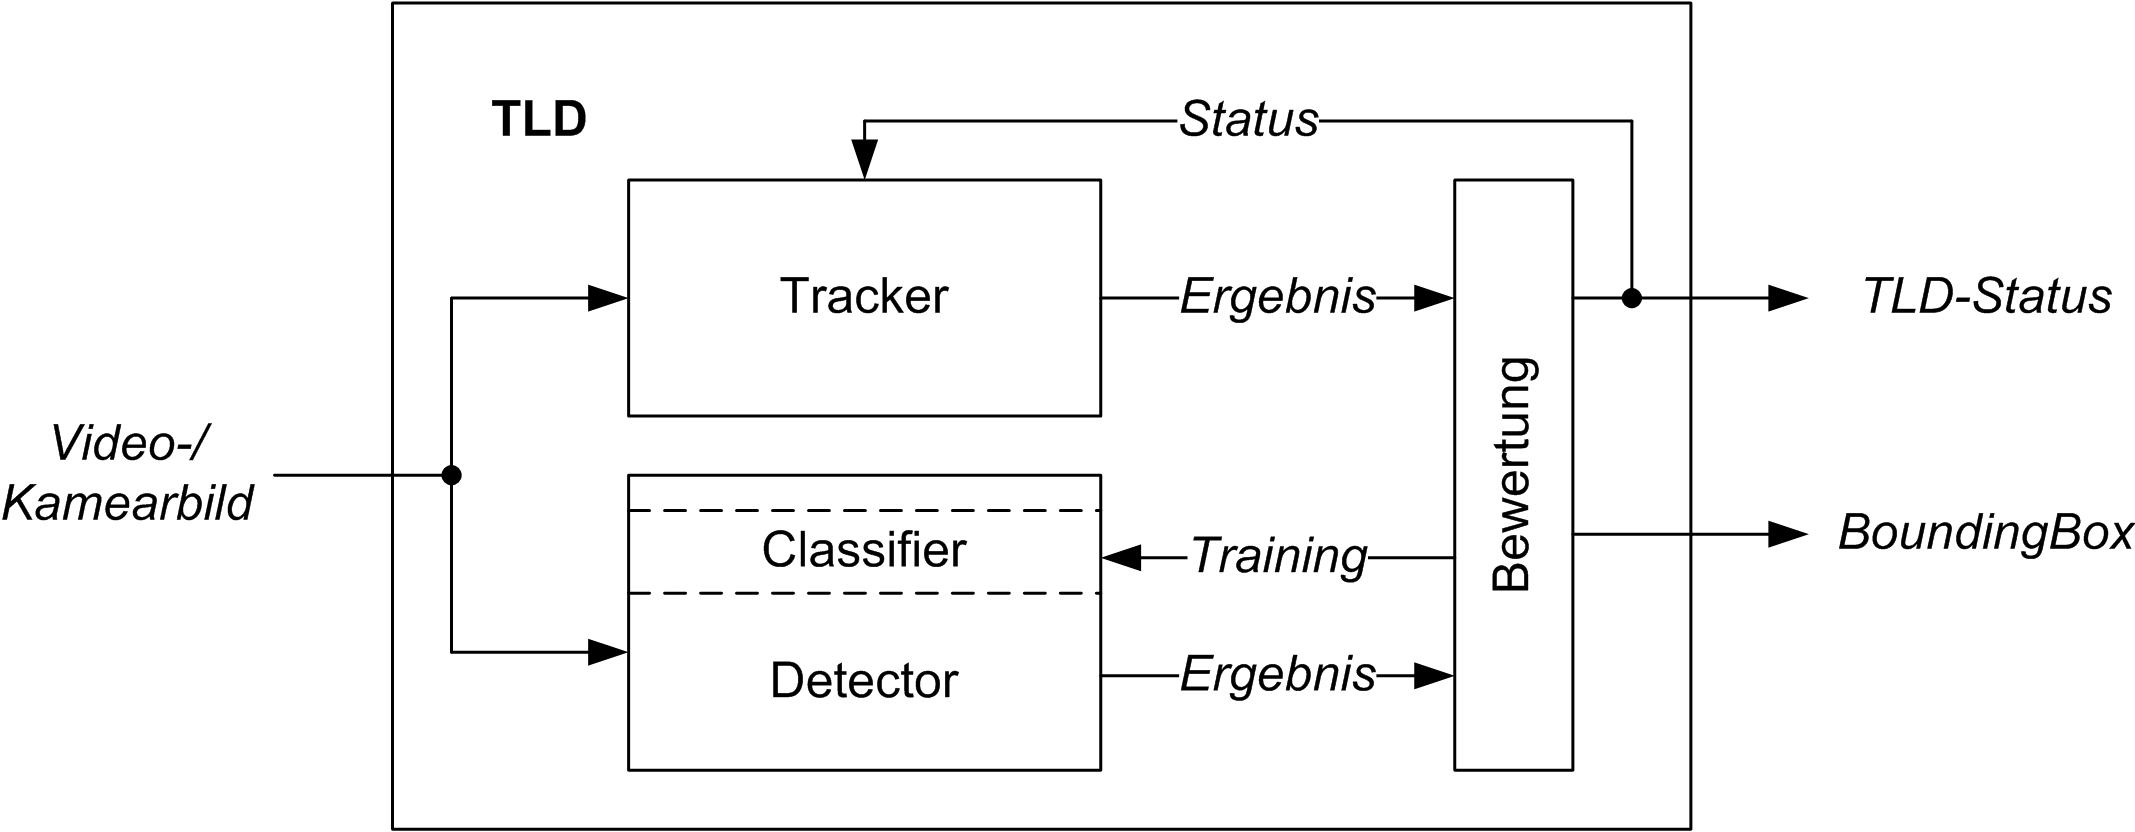
\includegraphics[scale=0.75]{../pictures/TLD-Framework.jpg}\caption{TLD-Schema}
\label{TLD-Schema}
\end{figure}

Als Sprache für die Umsetung wurde C++ gewählt, weil sie aufgrund der Möglichkeit relativ hardwarenah zu programmieren, schnelle Programme ermöglicht und durch OpenCV eine gut dokumentierte und umfangreiche Sammlung von Algorithmen speziell für den Bereich der Computer Vision liefert.

Im Anschluss zur Implementierung werden eine Reihe von Tests durchgeführt, die zu Beurteilung der Eignung von TLD für den speziellen Fall des Koptertrackings dienen. Es wird analysiert, welche Bedingungen zwingend gelten müssen, damit dieser Ansatz erfolgreich genutzt werden kann, und unter welchen Umständen sich TLD nicht eignet.


\subsection{Aufbau der Arbeit}
Die Arbeit ist wie folgt gegliedert.

\paragraph{Kapitel 1}
Das erste Kapitel stellt eine kurze Einführung in den Bereich der Computer Vision dar und leitet kurz den speziellen Bereich der Objekterkennung ein. Weiterhin wird die Zielsetzung der Arbeit definiert und der genutzte Algorithmus in Grundzügen vorgestellt.

\paragraph{Kapitel 2}
Dieses Kapitel gibt einen kurzen Überblick zu verwandten Arbeiten
und verschiedenen Ansätzen zur Lösung des Problems des machinellen Sehens. Unterschiedliche Paradigmen und deren Einsatzgebiete werden kurz vergleichend vorgestellt.


\paragraph{Kapitel 3 }
Hier erfolgt die genaue Beschreibung von TLD. Es werden ausführlich die theoretischen und mathematischen Hintergründe vorgestellt und der Algorithmus im Detail vorgestellt.

\paragraph{Kapitel 4}
Im vierten Kapitel wir kurz die C++-Implementierung beschrieben. Zusätzlich werden die verwendeten Testszenarien vorgestellt und die durchgeführten Tests beschrieben.

\paragraph{Kapitel 5}
Den Abschluss dieser Arbeit bildet dieses Kapitel der Auswertung und Analyse er Testergebnisse sowie eine Reihe von Vorschlägen für etwaige Verbesserungen.